Η επίλυση του συστήματος γίνεται με αριθμητική μέθοδο όπως έχει ήδη αναφερθεί. Καθώς η τα δεδομένα μπορεί να βασιστούν σε προσεγγίσεις, ενώ επίσης ολόκληρη η διαδικασία αποτελεί μια εκτίμηση, είναι φυσικό σε κάποια σημεία λειτουργίας, το μοντέλο να μη βρει δυνατές λύσεις εντός των περιορισμών. Για τον λόγο αυτό, επιλέχθηκε η χρήση αλγορίθμου ελαχιστοποίησης ($min(f)$), έναντι επίλυσης ισότητας (λ.χ \textit{Newton-Raphson}), ώστε σε αδύνατα σημεία του επιλύτη, να λάβουμε την κοντινότερη φυσική λύση που μπορεί να παράξει τη ζητούμενη κατάσταση.\\[10pt]

\noindent
Οι ελεύθερες μεταβλητές $\beta,\ \delta$ περιορίζονται ώστε να αποφευχθούν μη-φυσικές λύσεις.

\begin{equation*}
    \begin{aligned}
        \beta\ &\in\ [-15^\circ,15^\circ]\\
        \delta\ &\in\ [-45^\circ,45^\circ]       
    \end{aligned}
\end{equation*}

\subsubsection{Ορισμός αντικειμενικής συνάρτησης}

Ως αντικειμενική συνάρτηση επιλέγεται το τετράγωνο των υπολοίπων του συστήματος εξισώσεων (\ref{eq:stateSolverEquationSystem}).

\begin{equation}
    \left\{
    \begin{aligned}
        f_1(\mathbf{x}) &= \Biggl(M\dfrac{d}{dt}U_y(t) + M\dot{\psi}U_x - \sum_{i=FL,\dots,RR}\Bigl(F_{y,i}\Bigr)\Biggr)^2 \\[5pt]
        f_2(\mathbf{x}) &= \Biggl(\sum_{i=FL,\dots,RR} \Bigl(\vec{r}_i\times\vec{F}_i\Bigr)_z \Biggr)^2
    \end{aligned}
    \right.
    \label{eq:stateSolverResiduals}
\end{equation}

Επομένως, το πρόβλημα εμπίπτει στην ελαχιστοποίηση των αντικειμενικών συναρτήσεων $f_1(\mathbf{x}),f_2(\mathbf{x})$. Η επίλυση γίνεται μέσω της συνάρτησης \textit{lsqnonlin} της \textit{Matlab} \cite{mathworks_lsqnonlin}.

\subsubsection{Υλοποίηση περιορισμών}

Στους αλγορίθμους βελτιστοποίησης, η μέθοδος εφαρμογής των περιορισμών αποτελεί βασικότατο παράγοντα που επηρεάζει την ταχύτητα αλλά και την ικανότητα εύρεσης του βέλτιστου. Οι περιορισμοί δεν παίζουν απλά τον ρόλο της σήμανσης μιας λύσης ως ανέφικτη, αλλά βοηθούν τον αλγόριθμο να επιλέξει εφικτή λύση "στρίβοντας" τον προς τον εφικτό χώρο. Συνήθως αυτό επιτυγχάνεται με την επιβολή ποινής στην αντικειμενική συνάρτηση και χρησιμοποιούνται διάφορες προσεγγίσεις κλιμακοποίησης των ποινών \cite{nocedal2006numerical}. Στην υλοποίηση της παρούσας εργασίας, υπολογίζεται η τιμή της παραβίασης των περιορισμών και ο επιλύτης \textit{lsqnonlin} διαχειρίζεται την εφαρμογή των ποινών.
\noindent
\paragraph{Διαθέσιμη πρόσφυση ελαστικών}
Ο πρώτος περιορισμός είναι η δυνατότητα των ελαστικών να παρέχουν τα ζητούμενα φορτία. Όπως αναλύθηκε παραπάνω (\cref{eq:fxViolation}), η συνάρτηση του περιορισμού ορίζεται ως

\begin{equation}
    g_1(\mathbf{x}) = \sum_{i=FL,\dots,RR}\Bigl(F_{x,i,\text{έλλειμμα}}\Bigr)
\label{eq:totalFxViolation}
\end{equation}


\paragraph{Συνθήκη μη-ανατροπής}
Για την αποφυγή ανατροπής, ελέγχεται η ταυτόχρονη απώλεια κάθετου φορτίου σε
ζεύγη τροχών που ορίζουν πιθανό άξονα περιστροφής του οχήματος. Ορίζουμε το
σύνολο των κρίσιμων ζευγών
\begin{equation}
    \mathcal{P} = \bigl\{(FL,RL),\ (FR,RR),\ (FL,FR),\ (RL,RR)\bigr\},
\end{equation}
που αντιστοιχούν στην αριστερή και δεξιά πλευρά, καθώς και στον εμπρός και
πίσω άξονα. Για κάθε ζεύγος $(i,j)\in\mathcal{P}$, η συνεισφορά στη
συνάρτηση παραβίασης δίνεται ως

\begin{equation}
    \Pi_{(i,j)} =
    \begin{dcases}
        F_{z,i,\text{παραβ.}} + F_{z,j,\text{παραβ.}} & ,F_{z,i} < 0 \ \text{και}\ F_{z,j} < 0 \\
        0 & ,\text{σε κάθε άλλη περίπτωση}
    \end{dcases}
\end{equation}

και η συνολική συνεισφορά της συνθήκης μη-ανατροπής προκύπτει από την
άθροιση επί όλων των ζευγών,
\begin{equation}
    g_2(\mathbf{x}) = \sum_{(i,j)\in\mathcal{P}}\Pi_{(i,j)}
    \label{eq:noRolloverConstraint}
\end{equation}
Η διατύπωση αυτή επιτρέπει τη μεμονωμένη ανύψωση ενός τροχού --
αναμενόμενη κατάσταση σε έντονη εγκάρσια ή διαμήκη μεταφορά φορτίου -- χωρίς
να επιβάλλεται ποινή.

\subsection{Εξαγωγή αποτελεσμάτων}

\subsubsection{Μεταβλητές κατάστασης}

Το αποτέλεσμα της αριθμητικής επίλυσης είναι το ζεύγος γωνιών $\beta,\ \delta$ που ικανοποιούν τις εξισώσεις ισορροπίας σε μόνιμη κατάσταση. Χρησιμοποιώντας τη μεθοδολογία της ενότητας \ref{subsec:stateSolverEquations}, υπολογίζονται όλες οι μεταβλητές κατάστασης του πίνακα \ref{tab:stateUnknowns}.\\[10pt]

Παρακάτω παρατίθενται ενδεικτικά αποτελέσματα από επίλυση στην πίστα της Βαρκελώνης \textit{Circuit de Barcelona - Catalunya}. Σημειώνεται πως στο \cref{fig:carInCorner} οι γωνίες $\beta,\ \delta$ είναι αυξημένες για οπτικούς λόγους -- οι πραγματικές γωνίες δε θα ήταν ευδιάκριτες.

\begin{figure}[htbp!]
    \centering
    \begin{subfigure}[t]{0.32\textwidth}
        \centering
        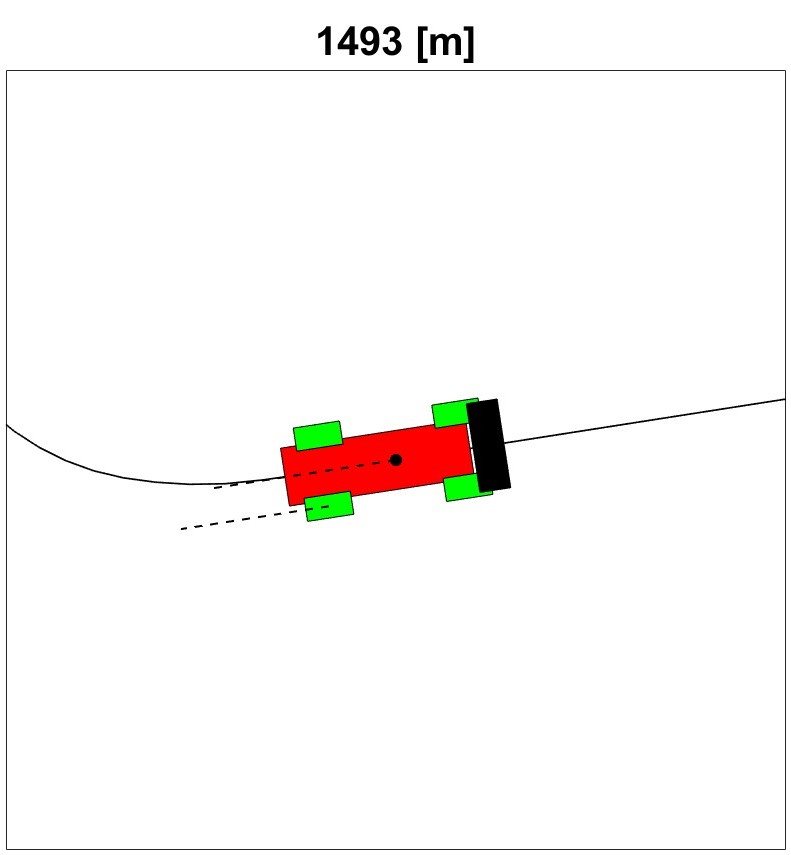
\includegraphics[height=5.5cm]{figures/curveEntry.jpg}
        \caption{Είσοδος στροφής}
        \label{fig:cornerEntry}
    \end{subfigure}
    \hfill
    \begin{subfigure}[t]{0.32\textwidth}
        \centering
        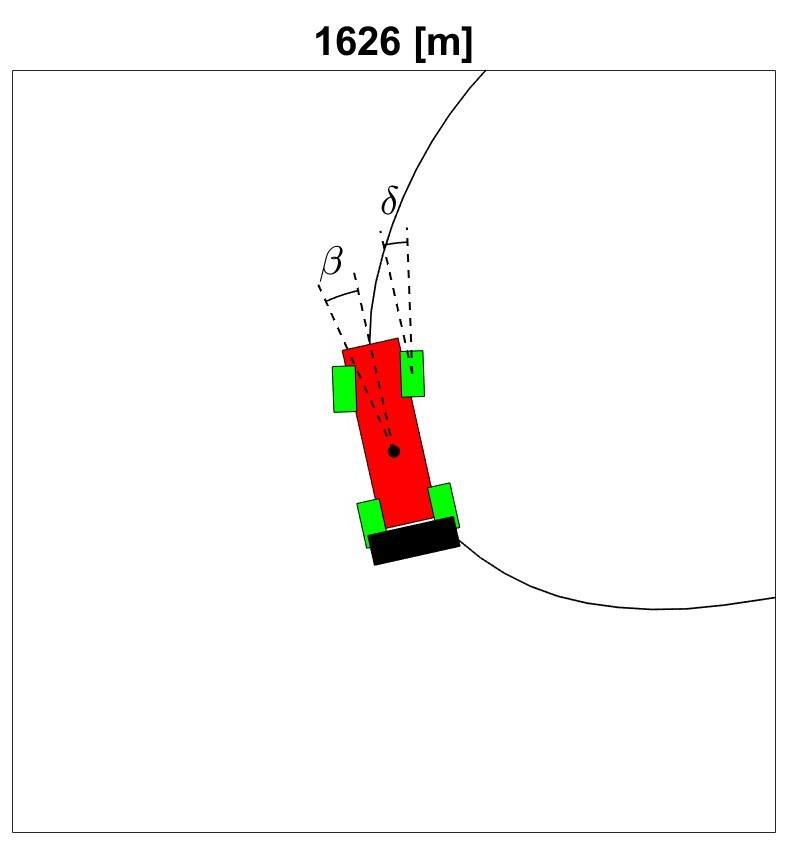
\includegraphics[height=5.5cm]{figures/curveMiddle.jpg}
        \caption{Μέσο στροφής}
        \label{fig:midCorner}
    \end{subfigure}
    \hfill
    \begin{subfigure}[t]{0.32\textwidth}
        \centering
        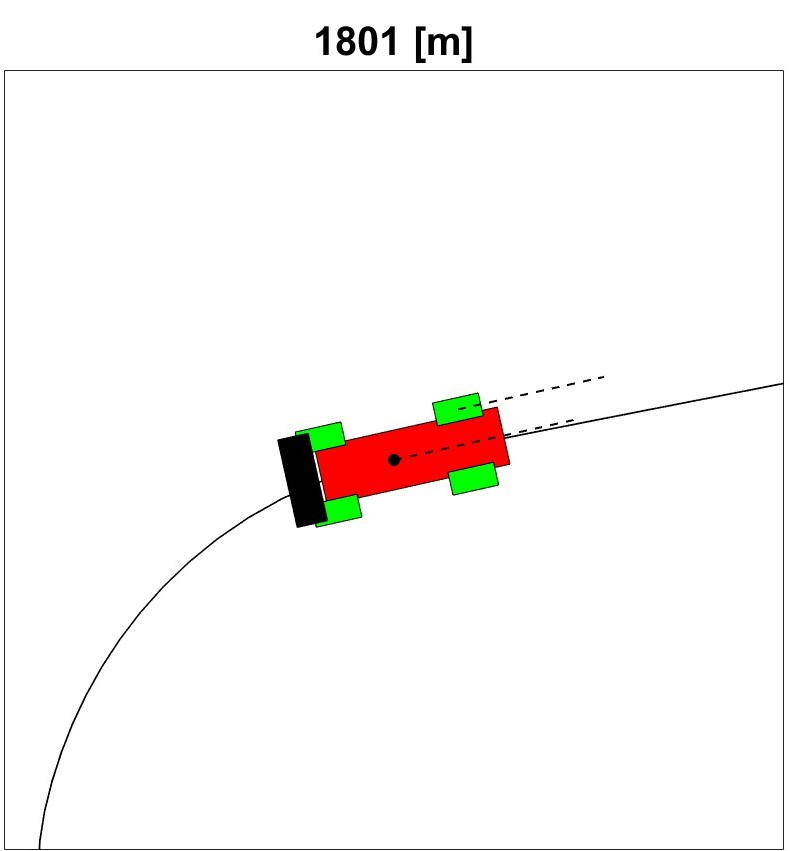
\includegraphics[height=5.5cm]{figures/curveExit.jpg}
        \caption{Εξοδος στροφής}
        \label{fig:cornerExit}
    \end{subfigure}
    \caption{Ενδεικτική σχηματική αναπαράσταση αποτελεσμάτων επίλυσης της κατάστασης οχήματος.}
    \label{fig:carInCorner}
\end{figure}


\begin{figure}[htbp!]
    \centering
    \begin{subfigure}[t]{0.48\textwidth}
        \centering
        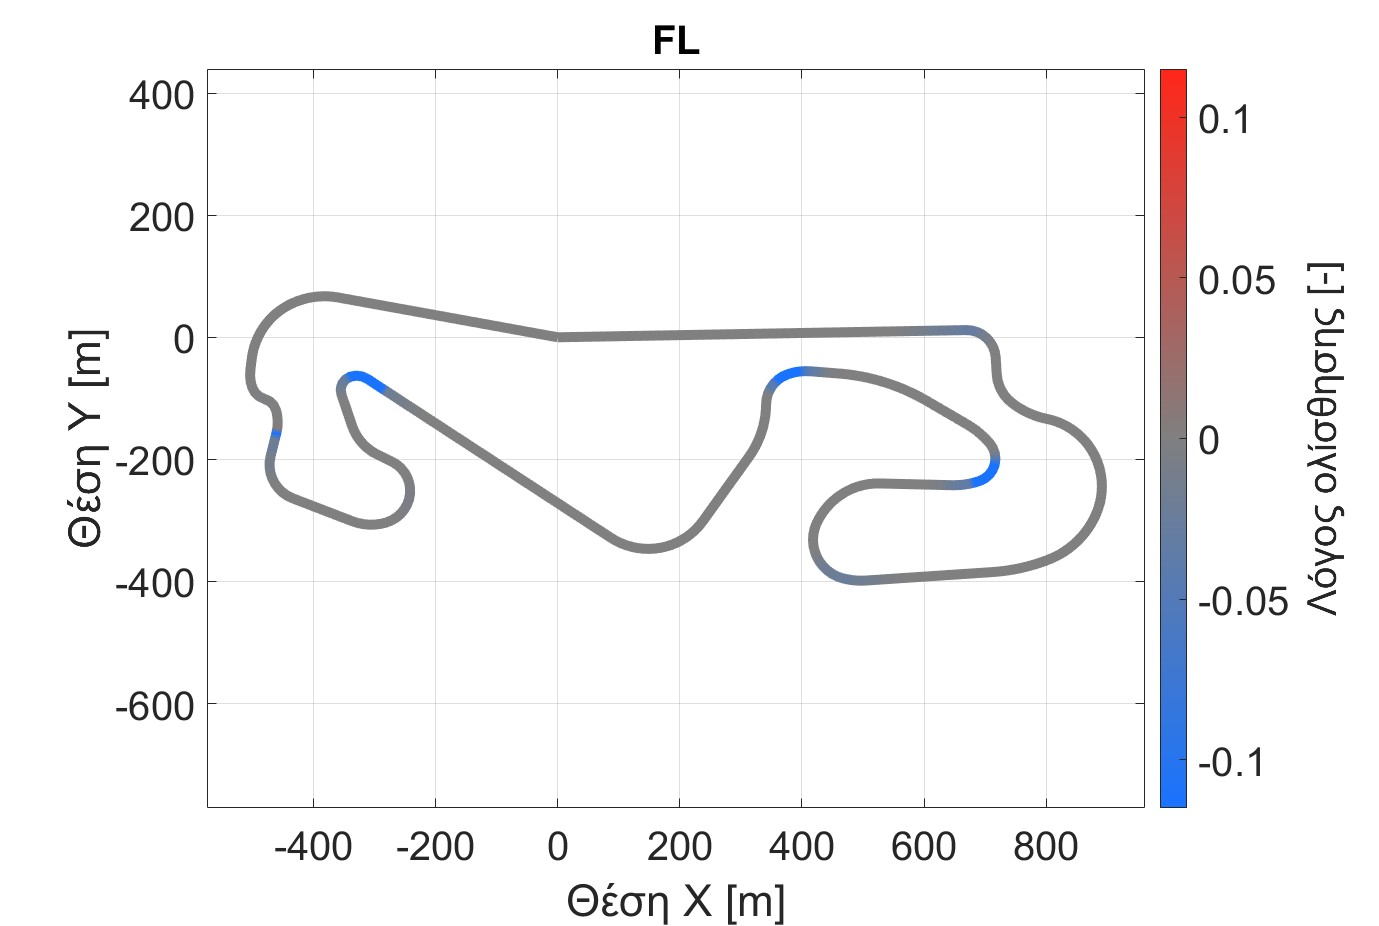
\includegraphics[width=\textwidth]{figures/slipRatioFL.jpg}
    \end{subfigure}
    \hfill
    \begin{subfigure}[t]{0.48\textwidth}
        \centering
        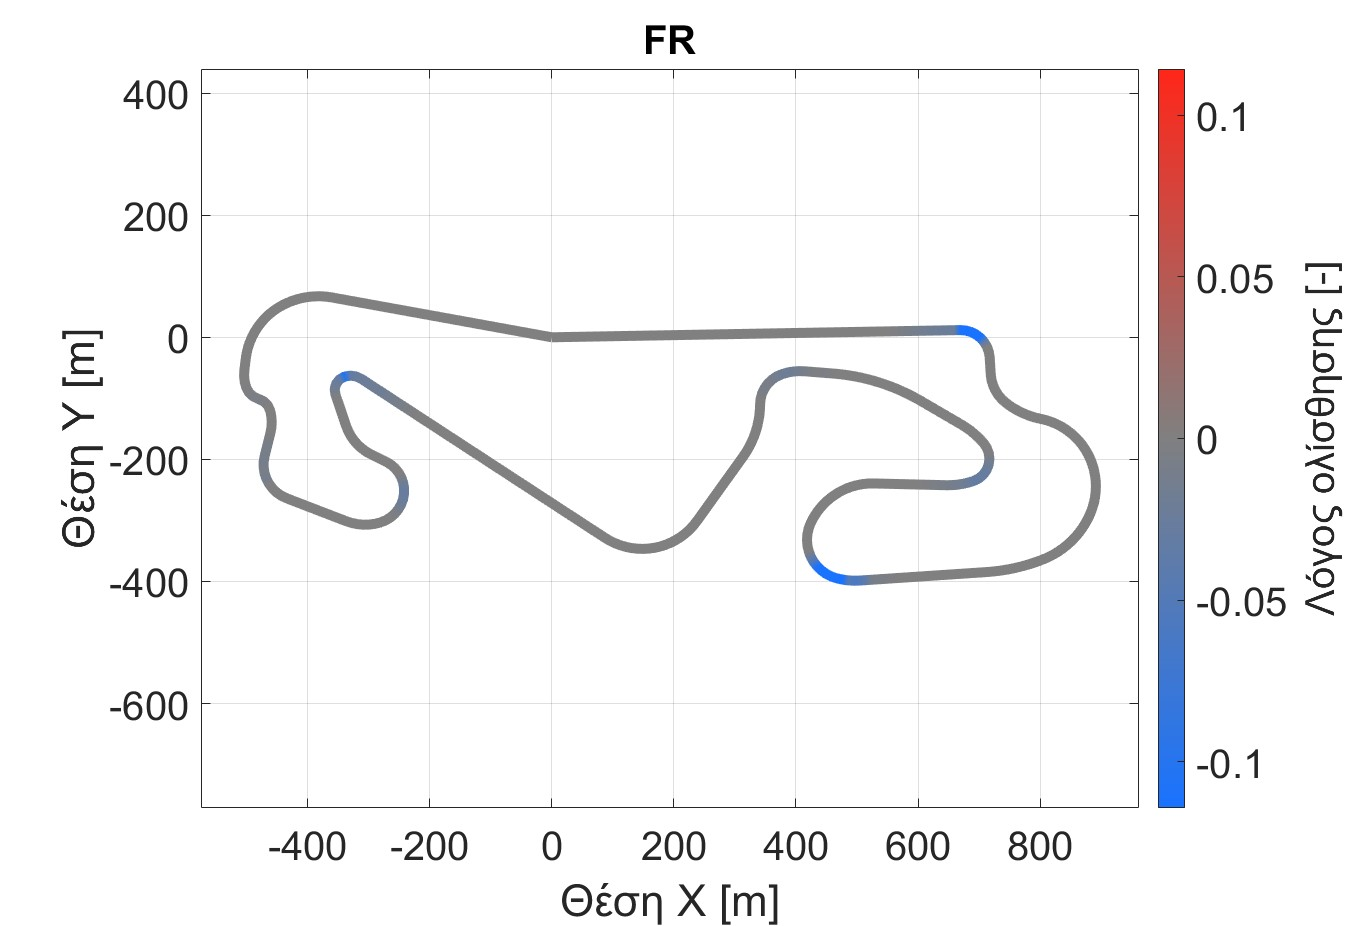
\includegraphics[width=\textwidth]{figures/slipRatioFR.jpg}
    \end{subfigure}

    \vspace{0.5em}

    \begin{subfigure}[t]{0.48\textwidth}
        \centering
        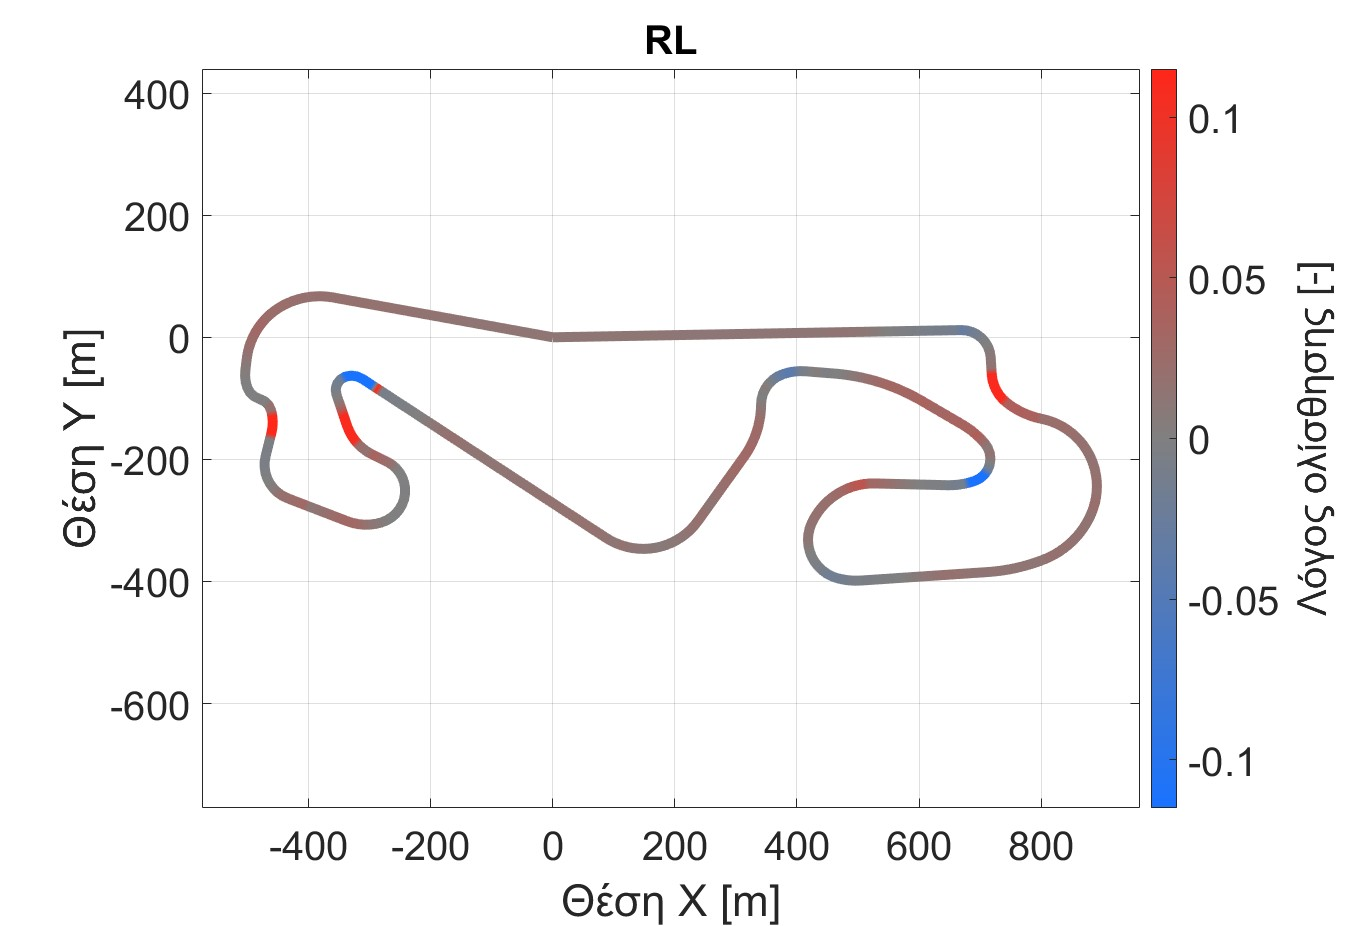
\includegraphics[width=\textwidth]{figures/slipRatioRL.jpg}
    \end{subfigure}
    \hfill
    \begin{subfigure}[t]{0.48\textwidth}
        \centering
        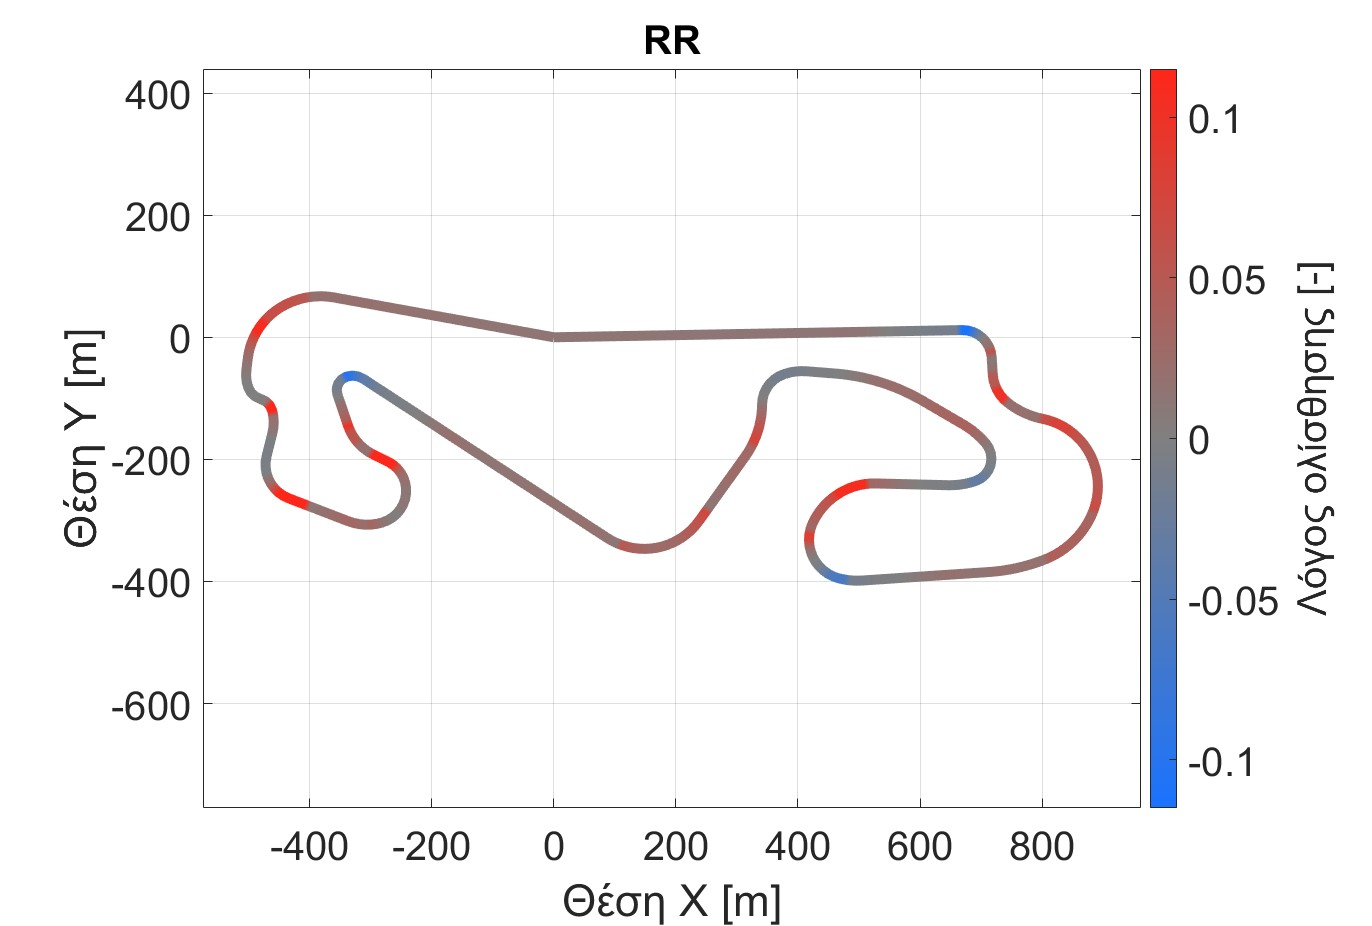
\includegraphics[width=\textwidth]{figures/slipRatioRR.jpg}
    \end{subfigure}
    \caption{Ενδεικτικά αποτελέσματα λόγου ολίσθησης σε γύρο της πίστας \textit{Circuit de Barcelona - Catalunya}}
    \label{fig:slipRatioSamples}
\end{figure}

\begin{figure}[htbp!]
    \centering
    \begin{subfigure}[t]{0.48\textwidth}
        \centering
        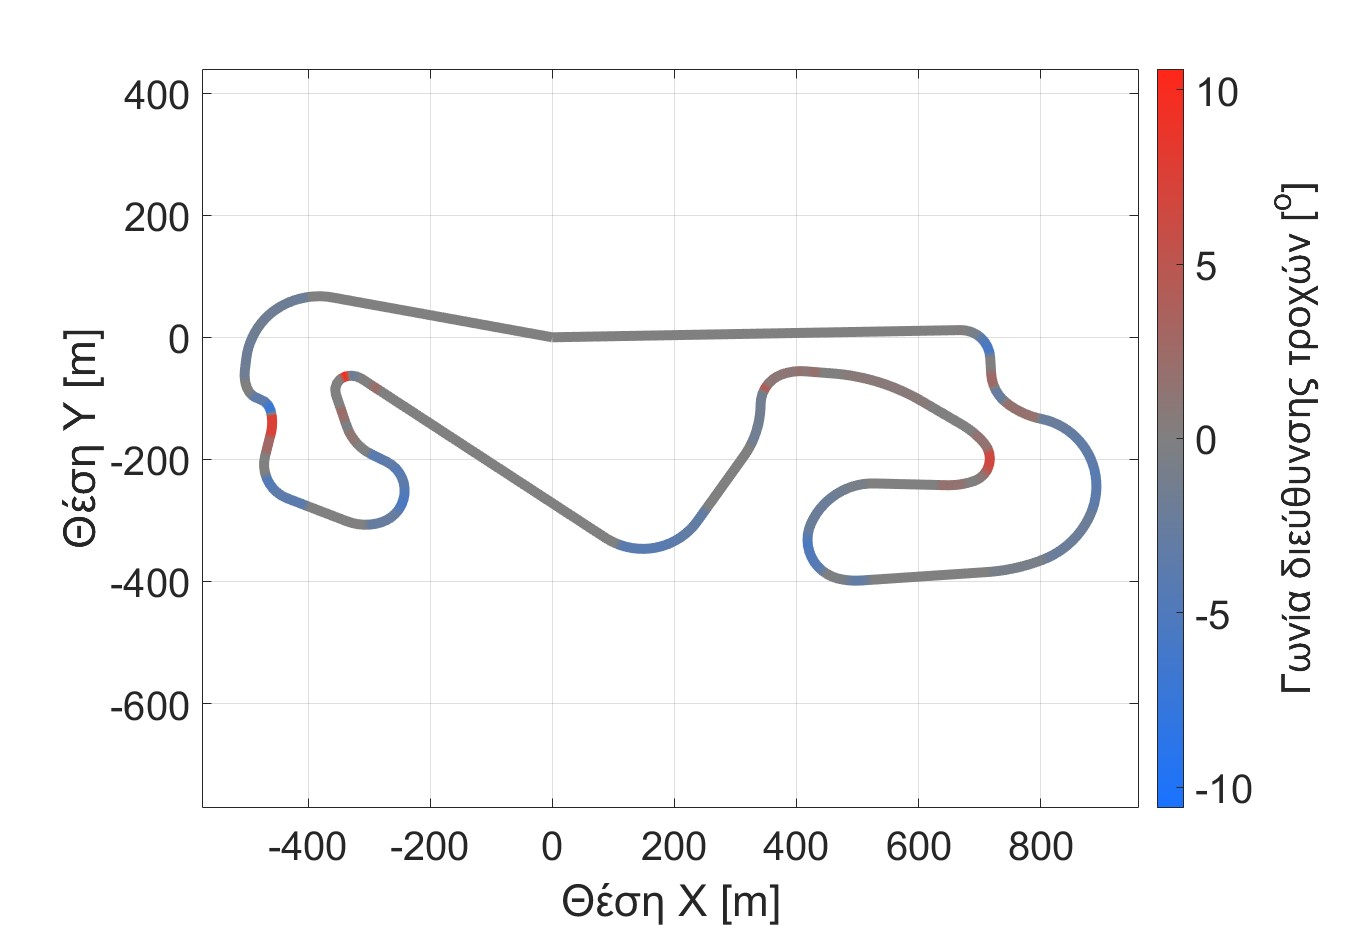
\includegraphics[width=\textwidth]{figures/steerAngle.jpg}
        \caption{Γωνία διεύθυνσης κατευθυντήριων τροχών}
        \label{fig:steerAnglePlot}
    \end{subfigure}
    \hfill
    \begin{subfigure}[t]{0.48\textwidth}
        \centering
        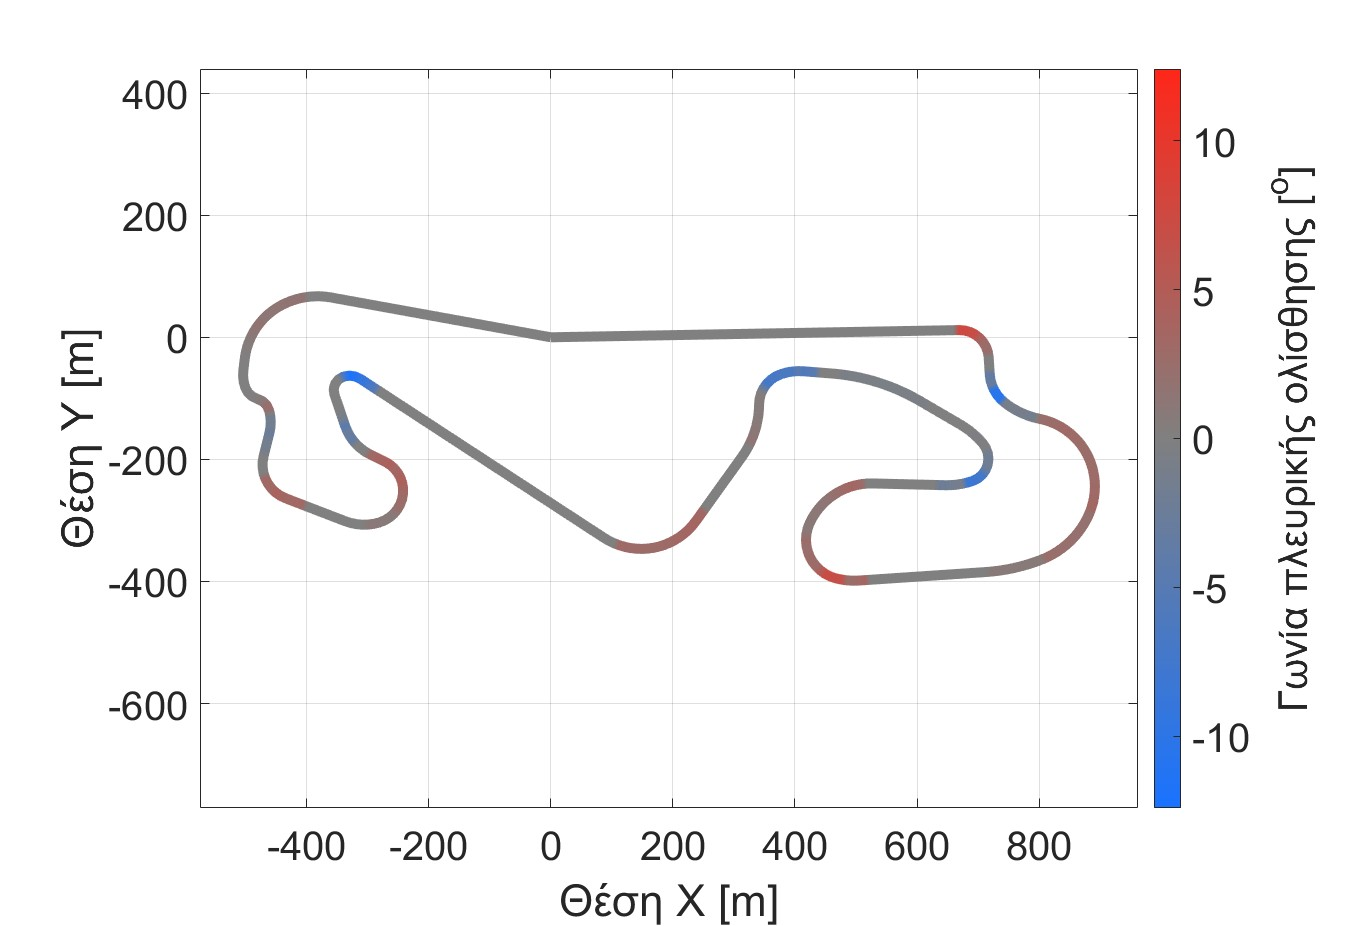
\includegraphics[width=\textwidth]{figures/chassisSlipAngle.jpg}
        \caption{Γωνία πλευρικής ολίσθησης}
        \label{fig:chassisSlipAnglePlot}
    \end{subfigure}
    \caption{Ενδεικτικά αποτελέσματα των μεταβλητών κατάστασης σε γύρο της πίστας \textit{Circuit de Barcelona - Catalunya}}
    \label{fig:solverAngles}
\end{figure}

\subsubsection{Θερμοκρασία και φθορά}

Σε αντίθεση με τις μεταβλητές κατάστασης του πίνακα \ref{tab:stateUnknowns}, η θερμοκρασία και η φθορά δε δίνονται μονοσήμαντα από τη δυναμική κατάσταση του οχήματος, αλλά περιλαμβάνουν την "ιστορία" του οχήματος καθώς αποτελούν ολοκληρώματα των αντίστοιχων ισχύων και ρυθμών φθοράς. Οι \cref{eq:dTds_full,eq:Wtotal} ολοκληρώνονται σε κάθε βήμα διακριτοποίησης της πίστας. Η ολοκλήρωση λαμβάνει χώρα σε κάθε σημείο της πίστας ταυτόχρονα με την επίλυση μόνιμης κατάστασης, καθώς η ανανεωμένη θερμοκρασία και φθορά επηρεάζουν τις καμπύλες πρόσφυσης των ελαστικών, και επομένως, επηρεάζουν την κατάσταση του οχήματος.

\paragraph{Θερμοκρασία}
Για την \cref{eq:dTds_full}, η οποία είναι διατυπωμένη ως προς την απόσταση $s$, εφαρμόζεται το κλασικό σχήμα \textit{Runge-Kutta} 4$^{\text{ης}}$ τάξης. Σε κάθε βήμα $s_n \rightarrow s_{n+1} = s_n + h$:

\begin{equation}
    \begin{aligned}
        k_1 &= \frac{1}{U_{x,n}}\,\dot{T}\!\left(\mathbf{x}_n,\ T_n\right)\\[2pt]
        k_2 &= \frac{1}{U_{x,n+\frac{1}{2}}}\,\dot{T}\!\left(\mathbf{x}_{n+\frac{1}{2}},\ T_n + \tfrac{h}{2}k_1\right)\\[2pt]
        k_3 &= \frac{1}{U_{x,n+\frac{1}{2}}}\,\dot{T}\!\left(\mathbf{x}_{n+\frac{1}{2}},\ T_n + \tfrac{h}{2}k_2\right)\\[2pt]
        k_4 &= \frac{1}{U_{x,n+1}}\,\dot{T}\!\left(\mathbf{x}_{n+1},\ T_n + h\,k_3\right)\\[2pt]
        T_{n+1} &= T_n + \frac{h}{6}\bigl(k_1 + 2k_2 + 2k_3 + k_4\bigr)
    \end{aligned}
    \label{eq:rk4Temperature}
\end{equation}

\noindent
όπου $\dot{T}$ ο ρυθμός μεταβολής θερμοκρασίας ως προς τον χρόνο και η διαίρεση με $U_x$ προκύπτει από τον κανόνα της αλυσίδας, ώστε η ολοκλήρωση να πραγματοποιείται ως προς την απόσταση. Οι ενδιάμεσες τιμές $\mathbf{x}_{n+\frac{1}{2}}$ των μεταβλητών κατάστασης του οχήματος προκύπτουν από γραμμική παρεμβολή μεταξύ των διαδοχικών σημείων διακριτοποίησης.

\paragraph{Φθορά}
Ο ρυθμός φθοράς είναι μονότονος και η ανά βήμα μεταβολή αμελητέα σε σχέση με το συνολικό πάχος του πέλματος, οπότε δεν απαιτείται σχήμα υψηλής τάξης. Η \cref{eq:Wtotal} ολοκληρώνεται ως προς τον χρόνο με σχήμα \textit{Euler}:

\begin{equation}
    W_{n+1} = W_n + \dot{W}_{n+1}\,\Delta t_{n+1}
    \label{eq:eulerWear}
\end{equation}

\noindent
όπου $\Delta t_{n+1} = t_{n+1} - t_n$ το χρονικό βήμα του τρέχοντος βήματος διακριτοποίησης.